% !Mode:: "Tex:UTF-8"
\chapter{基于余因子和Craig插值的迭代特征化算法}
\label{chap:interative_craig}



\section{引言}

在形式化验证和综合领域,
对于两个存在某种内在联系的逻辑向量$\vec{a}$和$\vec{b}$,
有两种不同的方式表达他们之间的联系:关系和函数。

其中,
关系$R(\vec{a},\vec{b})$更具一般性,
能够表达$\vec{a}$和$\vec{b}$之间的任意对应。
尤其是一对多的对应,
这是关系比函数具有更强描述能力的地方。
这种一般性在形式化验证中广泛用于描述非确定性行为以扩展描述能力\upcite{nda},
以及构造抽象模型\upcite{DBLP:conf/cav/ClarkeGJLV00}以削减计算复杂性等。

而另一方面,
函数是关系的一种受限形式。
如果$R(\vec{a},\vec{b})$满足以下要求,
则能将其转换为相应的函数$\vec{b}:=f(\vec{a})$:
对$\vec{a}$的任意取值$x\in[\![\vec{a}]\!]$,
均存在且仅存在唯一的$y\in[\![\vec{b}]\!]$,
使得$R(\vec{a},\vec{b})$。
在实际的软硬件设计与验证领域,
存在大量的情况需要从一个关系中获得相应的函数。
如在自动激励生成算法中从约束描述产生相应的激励函数\upcite{DBLP:conf/dac/YuanAAP03},
证明导引抽象中的抽象模型构造\upcite{DBLP:conf/fmcad/AmlaM04},
以及本文中推导控制流谓词和特征化解码器等。

以图\ref{fig_relation}为例。
对于图\ref{fig_relation}a)中的一对一映射,
我们可以使用布尔函数$y_1=x_1\wedge x_2$和$y_2=\neg x_1\wedge \neg x_2$表示。
而另一方面,
对于图\ref{fig_relation}b)中的布尔关系,
并不存在相应的布尔函数,
因为$(x_1,x_2)=(0,1)$的情形被映射到了多个$(y_1,y_2)$的组合。
而这种情况可以使用布尔关系$R=(\neg x_1\wedge\neg x_2\wedge \neg y_1\wedge y_2)
\vee(\neg x_1\wedge x_2\wedge \neg y_1\wedge \neg y_2)
\vee(\neg x_1\wedge x_2\wedge y_1\wedge y_2)
\vee(x_1\wedge \neg x_2\wedge \neg y_1 \wedge \neg y_2)
\vee(x_1\wedge x_2\wedge y_1\wedge \neg y_2)$。

\begin{figure}[t]
\begin{center}
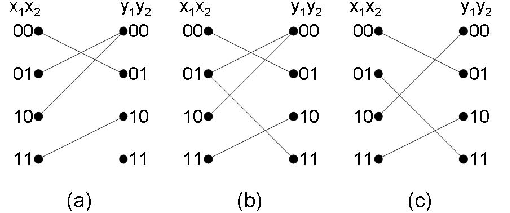
\includegraphics[width=0.8\textwidth]{relation}
\end{center}
\caption{关系和函数的布尔映射}
  \label{fig_relation}
\end{figure}

为此,
我们在本章中提出了基于余因子和Craig插值的迭代特征化算法,
以从布尔关系$R(\vec{a},\vec{b},t)$中特征化函数$t=f(\vec{a})$。

在本章中,
我们首先在小节\ref{sec_craigimp}描述Craig插值的基本原理,
然后在小节\ref{sec_craigchar}中将其应用至一种受限的特殊情况下以求解特征化函数。
最后在小节\ref{sec_iterativecraig}中将其扩展到包含额外变量$\vec{c}$ 的更一般情形$R(\vec{a},\vec{b},\vec{c})$。

\section{Craig插值的原理和实现}\label{sec_craigimp}
注意本小节描述的Craig插值原理不是我们的原创,
而是为了方便上下文的叙述从\upcite{DBLP:conf/cav/McMillan03} 移植至此。
\subsection{相关背景知识和记法}
在通常的SAT求解器,
包括本文使用的MiniSat\upcite{EXTSAT}中,
要求待求解的公式被表示为CNF格式。
其中一个公式是多个短句的合取(conjunction),
而每一个短句是多个文字的析取(disjunction),
而每个文字是一个布尔变量$v$或者其反$\neg v$。
如公式$(v_0\vee\neg v_1\vee v_2)\wedge(v_1\vee v_2)\wedge(\neg v_0\vee v_2)$,
包含短句$v_0\vee\neg v_1\vee v_2$,$v_1\vee v_2$和$\neg v_0\vee v_2$。
而短句$v_0\vee\neg v_1\vee v_2$包含文字$v_0$, $\neg v_1$和$v_2$。

当存在一个变量$v$,
使得一个短句$c$中同时包含两个文字$v$和$\neg v$,
则称$c$为tautological的。
我们通常假设有待SAT求解器求解的公式中所有的短句都是非tautological的。

假设公式$F$的布尔变量全集为$V$。
若存在对$V$的赋值函数$A:V\to \{0,1\}$,
使得$F$中的每个短句均能取值为1,
则称$F$是可满足的,
此时SAT求解器能够找到赋值函数$A$。
否则称$F$为不可满足的,
此时SAT求解器能够产生如下一小节所述的不可满足证明。

\subsection{不可满足证明}
对于两个短句$c_1=v\vee B$和$c_2=\neg v\vee C$,
当$A\vee B$是非tautological的时,
$A\vee B$称为他们的resolvant。
而$v$称为他们的pivot。
易知以下事实:

\begin{equation}
\begin{array}{ccc}
&resolvant(c_1,c_2) = \exists v, c_1\wedge c_2 &\\
&c_1\wedge c_2 \to resolvant(c_1,c_2)&
\end{array}
\end{equation}

\begin{definition}
对于不可满足公式$F$,
假设其短句集合为$C$,
则其不可满足证明$\Pi$是一个有向无环图$(V_{\Pi},E_{\Pi})$,
其中$V_{\Pi}$是短句集合,
而$E_{\Pi}$是链接$V_{\Pi}$中节点的边集合。
$\Pi$满足如下要求:
\begin{enumerate}
\item 对于节点$c\in V_{\Pi}$:
  \begin{enumerate}
    \item 要么$c\in C$,此时称$c$为$\Pi$的根
    \item 或者$c$有且仅有两个predecessors $c_1$和$c_2$,
    使得$c$是$c_1$和$c_2$的resolvant。
  \end{enumerate}
\item 空短句是$\Pi$的唯一一个叶节点。
\end{enumerate}
\end{definition}

直观的说,
$\Pi$就是一棵树,
以短句集合$C$的子集为根,
以空短句为唯一叶节点。
而每个节点的两个扇入边代表了一个resolving关系。

包括本文使用的MiniSat求解器\upcite{EXTSAT}在内的许多SAT求解器,
当公式不可满足时都将产生一个不可满足证明$\Pi$。

\subsection{Craig插值算法}

根据文献\upcite{Craig},
给定两个布尔逻辑公式$A$ 和$B$,
若$A\wedge B$ 不可满足,
则存在仅使用了$A$ 和$B$共同变量的公式$I$ ,
使得$A\Rightarrow I$且
$I\wedge B$不可满足。
$I$ 被称为$A$针对$B$的Craig插值\upcite{Craig}。

目前最常见且最高效的产生Craig插值的算法是
McMillan算法\upcite{interp_McMillan} 。
其基本原理描述如下。

对于上述公式$A$和$B$,
已知$A\cup B$不可满足,
而$\Pi$是SAT求解器给出的不可满足证明。
当一个变量$v$同时出现在$A$和$B$中时,
我们称其为全局变量。
若$v$只出现在$A$中,
则称其为$A$本地变量。

对于文字$v$或者$\neg v$,
当变量$v$是全局变量或者$A$本地变量时,
称该文字为全局文字或者$A$本地文字。

对于短句$c$,
令$g(c)$为$c$中所有全局文字的析取,
而$l(c)$为$c$中所有$A$本地文字的析取。

例如,
假设有两个短句$c_1=(a\vee b\vee\neg c)$ 和
$c_2=(b\vee c\vee\neg d)$。
并假设$A=\{c_1\}$和$B=\{c_2\}$。
则$g(c_1)=(b\vee\neg c)$,
$l(c_1)=(a)$,
$g(c_2)=(b\vee c)$,
$l(c_2)=FALSE$。


\begin{definition}\label{def_gencraig}
令$(A,B)$为一对公式,
而$\Pi$是$A\cup B$的不可满足证明,
且其唯一叶节点是空短句$FALSE$。
对于每一个节点$c\in V_{\Pi}$,
令$p(c)$为如下定义的一个公式:
\begin{enumerate}
\item 如果$c$是根节点则
  \begin{enumerate}
    \item 如果$c\in A$则$p(c)=g(c)$
    \item 否则$p(c)=TRUE$
  \end{enumerate}
\item 否则令$c_1$和$c_2$分别是$c$的两个扇入节点,而$v$是他们的pivot变量
  \begin{enumerate}
    \item 如果$v$是$A$本地变量,则$p(c)=p(c_1)\vee p(c_2)$。
    \item 否则$p(c)=p(c_1)\wedge p(c_2)$。
  \end{enumerate}
\end{enumerate}
\end{definition}

上述定义\ref{def_gencraig}是构造性的,
已经给出了从$\Pi$得到最终的插值的算法,
即以$\Pi$的根节点为起点,
为每一个$c$计算相应的$p(c)$,
直至到达最终的唯一叶节点$FALSE$。
我们有以下定理:

\begin{theorem}
定义\ref{def_gencraig}为唯一叶节点$FALSE$产生的$p(FALSE)$即为
$A$相对于$B$的Craig插值。
\end{theorem}

该定理的详细证明可见文献\upcite{DBLP:journals/tcs/McMillan05}。

计算$A$相对于$B$的Craig插值的时间复杂性为$O(N+L)$,
其中$N$是$\Pi$中包含的节点个数$|V_{\Pi}|$,
而$L$是$\Pi$中的文字个数$\sigma_{c\in V_{\Pi}}|c|$。
而所产生的插值可以视为一个电路,
其空间复杂性为$|O(N+L)|$。
当然,
$\Pi$的尺寸在最坏情况下也是$A\cup B$的尺寸的指数。



\section{非迭代的特征化算法}\label{sec_craigchar}

假设有布尔关系$R(t,\vec{a})$使得
$R(1,\vec{a})\wedge R(0,\vec{a})$不可满足。
而我们需要从$R$中特征化函数$f$,
使得$t=f(\vec{a})$。
则根据上述的讨论,
可以简单的令$A=R(1,\vec{a})$而$B=R(0,\vec{a})$。
此时$A$相对于$B$的Craig插值$\Pi$具有以下性质:

\begin{enumerate}
\item $R(1,\vec{a})\to \Pi$,这说明$\Pi$覆盖了所有能够使得$R(1,\vec{a})$的$\vec{a}$。
\item $R(0,\vec{a})\wedge \Pi$不可满足,这说明$\Pi$没有覆盖任何使得$R(0,\vec{a})$的$\vec{a}$。
\item $\Pi$仅引用了$R(0,\vec{a})$和$R(1,\vec{a})$的共同变量集合$\vec{a}$。这说明$\Pi$是一个定义在$\vec{a}$上的函数。
\end{enumerate}

因此,
$\Pi$即为函数$f$。

该算法在本文的后继章节中被广泛应用于构造解码器的布尔函数。


\section{迭代的特征化算法}\label{sec_iterativecraig}
上一小节讨论了如何从关系$R(a,\vec{b})$特征化函数$a=f(\vec{b})$。
然而在更一般的情形下,我们需要从$R(\vec{a},\vec{b},t)$特征化函数$t=f(\vec{a})$。
相比之下,此时多了一个需要进行存在性量化的$\vec{b}$。
为此我们需要将上述算法进行以下扩展。

假设$R(\vec{a},\vec{b},t)$是一个使得$R(\vec{a},\vec{b},0)\wedge R(\vec{a},\vec{b},1)$ 不可满足的布尔公式。

其中$\vec{a}$ 和$\vec{b}$ 被分别称为重要和非重要变量子集。
而$t$ 是目标变量。
我们进一步假设$R(\vec{a},\vec{b},t)$ 是可满足的。

我们需要特征化一个布尔函数$FSAT_R(\vec{a})$,
覆盖且仅覆盖了所有能够使得$R(\vec{a},\vec{b},1)$ 可满足的$\vec{a}$。
形式化的定义是:

\begin{equation}\label{fchar}
% \begin{split}
FSAT_R(\vec{a}):=
\left\{
\begin{array}{rcl}
1 & & \exists\vec{b}.R(\vec{a},\vec{b},1) \\
0 & & otherwise
\end{array}
\right.
% \end{split}
\end{equation}
%% HAHA come to here

因此,
一个计算$FSAT_R(\vec{a})$ 的简单算法是:
逐一遍历并收集所有使得$R(\vec{a},\vec{b},1)$ 可满足的$\vec{a}$的赋值。
然而该算法需要处理$2^{|\vec{a}|}$中情况。
对于很长的$\vec{a}$,时间开销将会很大。

使用cofactoring \upcite{EFFSATUSMCCO} 和Craig 插值\upcite{interp_McMillan},
可以将每一个$\vec{a}$ 扩展为一个更大的集合,
从而极大的提高算法运行速度。
直观的,
假设$R(\vec{a},\vec{b},1)$ 的一个满足赋值是$A:\vec{a}\cup\vec{b}\cup\{t\}\to\{0,1\}$,
通过cofactoring\upcite{EFFSATUSMCCO}可以构造以下公式:

\begin{algorithm}[t]
\caption{$CharacterizingFormulaSAT(R,\vec{a},\vec{b},t)$: 特征化使得$R(\vec{a},\vec{b},1)$ 可满足的$\vec{a}$ 集合}
\label{alg_craigchar}
%\KwIn{The Boolean formula $R(\vec{a},\vec{b},t)$,
%its important variable vector $\vec{a}$,
%its non-important variable vector $\vec{b}$,
%and its target variable $t$.}
%\KwOut{$FSAT_R(\vec{a})$ that makes $R(\vec{a},\vec{b},1)$ satisfiable.}
\begin{algorithmic}[1]
\label{initcondition}
\STATE $FSAT_R(\vec{a}):= 0$ ;
\WHILE { $R(\vec{a},\vec{b},1)\wedge\neg FSAT_R(\vec{a})$ 是可满足的}
\label{testsat}
  \STATE 假设 $A:\vec{a}\cup\vec{b}\cup\{t\}\rightarrow \{0,1\}$ 可满足赋值函数;
  \STATE $\phi_A(\vec{a}):= R(\vec{a},A(\vec{b}),1)$ ;
\label{cofact1}
  \STATE $\phi_B(\vec{a}):= R(\vec{a},A(\vec{b}),0)$ ;
\label{cofact2}
  \STATE 假设 $ITP(\vec{a})$ 是$\phi_A$ 针对$\phi_B$的Craig插值 ;
\label{ab}
  \STATE $FSAT_R(\vec{a}):= ITP(\vec{a}) \vee FSAT_R(\vec{a})$ ;
\label{add}
\ENDWHILE
\RETURN $FSAT_R(\vec{a})$
\end{algorithmic}
\end{algorithm}

\begin{equation}
% \begin{split}
R(\vec{a},A(\vec{b}),1):=R(\vec{a},\vec{b},1)_{b\equiv A(b)}
% \end{split}
\end{equation}

因为$R(\vec{a},A(\vec{b}),0)\wedge R(\vec{a},A(\vec{b}),1)$ 是不可满足的,
$R(\vec{a},A(\vec{b}),1)$针对$R(\vec{a},A(\vec{b}),0)$的Craig插值$ITP(\vec{a})$ 可以用作$\vec{a}$ 使得$R(\vec{a},A(\vec{b}),1)$ 可满足的上估计。
同时,
$ITP(\vec{a})\wedge R(\vec{a},A(\vec{b}),0)$ 是不可满足的,
因此$ITP(\vec{a})$ 没有覆盖任何使得$R(\vec{a},A(\vec{b}),0)$ 可满足的情况。
因此,
$ITP(\vec{a})$ 覆盖且仅覆盖了所有使得$R(\vec{a},A(\vec{b}),1)$ 可满足的$\vec{a}$。


基于上述讨论,
我们提出了算法\ref{alg_craigchar} 以特征化等式(\ref{fchar})中的$FSAT_R(\vec{a})$。
行\ref{testsat}检测是否仍然存在尚未被$FSAT_R(\vec{a})$覆盖的$\vec{a}$ ,
使得$R(\vec{a},\vec{b},1)$ 可满足。
行\ref{cofact1} 和\ref{cofact2} 将可满足赋值中$\vec{b}$的取值分别赋予
$R(\vec{a},\vec{b},1)$ 和$R(\vec{a},\vec{b},0)$ 。
这将使得$\vec{b}$ 不在出现在这两个公式中。

因此,
$\phi_A\wedge \phi_B$ 在行\ref{ab} 是不可满足的。
且$\phi_A$ 和$\phi_B$ 的共同变量是$\vec{a}$。
因此可以使用McMillian算法\upcite{interp_McMillan} 计算Craig 插值$ITP(\vec{a})$。

$ITP(\vec{a})$ 将在行\ref{add}被加入$FSAT_R(\vec{a})$  并在行\ref{testsat} 被排除。

算法\ref{alg_craigchar} 的每一个循环将向$FSAT_R(\vec{a})$ 中加入至少一个$\vec{a}$ 的赋值。
这意味着$FSAT_R(\vec{a})$ 覆盖了$\vec{a}$的一个有界并且单调增长的赋值集合。
因此算法\ref{alg_craigchar} 是停机的。

\section{本章小结}
本章综述了Craig插值算法的原理及其实现,
以及基于该实现的迭代是特征化算法。
这些算法将在本文的剩余部分被其他算法频繁调用。


